\section{Introduction}

A new dispersion modeling system based on the well-used FORTRAN-based QUIC (Quick Urban and Industrial Complex) dispersion modeling system originally developed by the University of Utah and Los Alamos National Laboratory \cite{brown2013quic}, has been under development as collaboration between the University of Utah, the University of Minnesota, Duluth and Pukyong National University. Quick Environmental Simulation (QES) is a microclimate simulation platform for computing 3D environmental scalars in urban areas and over complex terrain. QES-Winds, QES-TURB and QES-Plume are mean wind modeling, turbulence, and plume dispersion modeling components of QUIC EnvSim (QES). Figure below shows a schematic of QES system and how different elements of the system interact with each other.

\begin{figure}[h!]
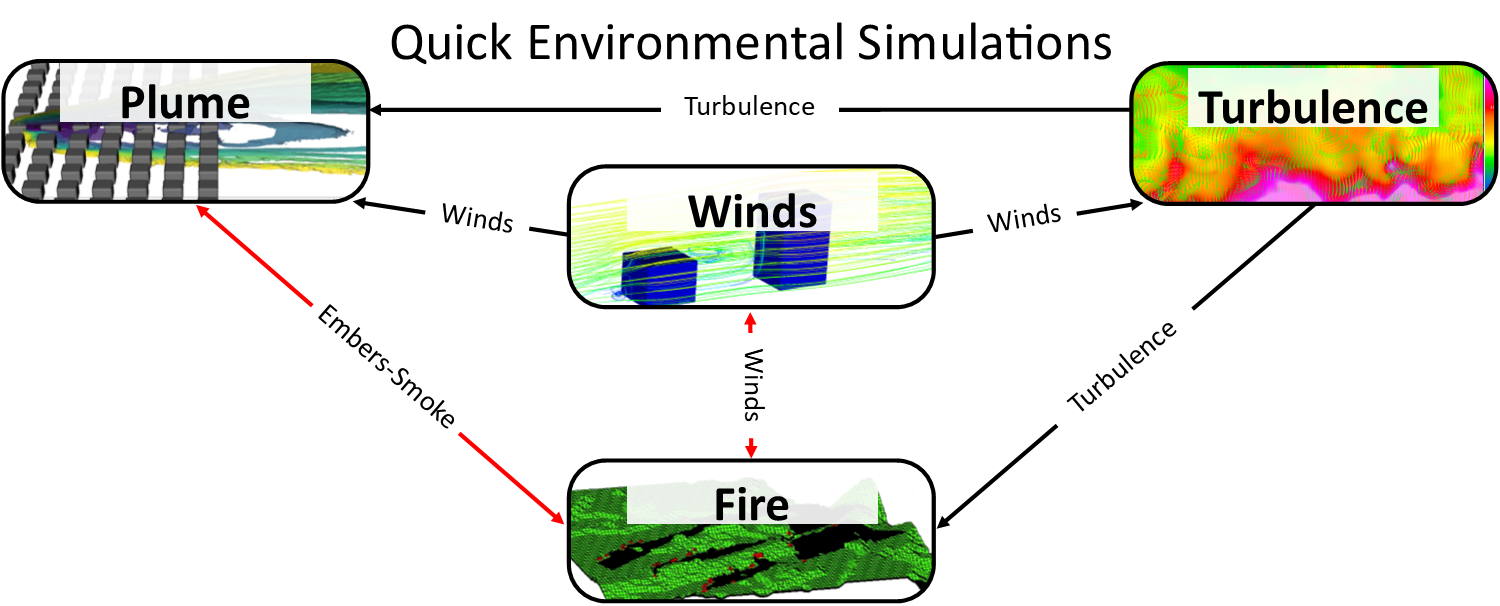
\includegraphics[width=16cm]{Images/QES_chart.png}
\centering
\caption{Schematic of the QUIC EnvSim system and the relationship between different elements of the system including data flow from one element to the other}
\end{figure}

The QES code is a low-computational-cost framework designed to compute high-resolution wind and concentration fields in complex atmospheric-boundary-layer environments. QES is written in C++ and NVIDIA's CUDA for Graphics Processing Unit (GPU) acceleration. The code uses NVIDIA's dynamic parallelism API to substantially accelerate simulations. \textbf{QES requires a NVIDIA GPU with Compute Capability of 7.0 (or higher)}.


\subsection{QES-Winds}

QES-Winds is a fast-response 3D diagnostic urban wind model using a mass-conserving wind-field solver \cite{Bozorgmehr2021}. QES-Winds uses a variational analysis technique to ensure the conservation of mass rather than slower yet more physics-based solvers that include the conservation of momentum. QES-Winds minimizes the difference between an initial wind field that is specified using empirical parameterizations and the final wind field. This method requires the solution of a Poisson equation for Lagrange multipliers. The Poisson equation is solved using the Successive Over-Relaxation (SOR) method (an iterative solver), which is a variant of the Gauss-Seidel method with more rapid convergence.

\subsection{QES-Turb}

QES-Turb is a turbulence model based on Prandtl’s mixing-length and Boussinesq eddy-viscosity hypotheses. QES-Turb computes the stress tensor using local velocity gradients and some emprical non-local parameterizations.

\subsection{QES-Plume}

QES-Plume is a stochastic Lagrangian dispersion model using QES-Winds mean wind field and QES-Turb turbulence fields. QES-Plume solves the generalized Langevin equations to compute the fluctuations of the particle in the turbulent flow fluid. A time-implicit integration scheme is used to solve the Langevin equation, eliminating 'rogue' trajectories. The particles are advanced using a forward Euler scheme. QES-Plume is also a stand-alone dispersion model that can run using fields from diverses sources such as RANS or LES models.


\subsection{QES-Fire}

QES-Fire is a microscale wildfire model coupling the fire front to microscale winds. The model consists of a simplified physics rate of spread model, a kinematic plume-rise model, and a mass-consistent wind solver. The QES-Fire module is currently not publicly available.


\subsection{Publications}

\begin{itemize}

\item QES-Winds: Dynamic Parallelism Solver

Bozorgmehr, B., Willemsen, P., Gibbs, J.A., Stoll, R., Kim, J.-J., Pardyjak, E.R., 2021. Utilizing dynamic parallelism in CUDA to accelerate a 3D red-black successive over relaxation wind-field solver. Environ Modell Softw 137, 104958. https://doi.org/10.1016/j.envsoft.2021.104958

\item QES-Winds: Isolated Tree Model

Margairaz, F., Eshagh, H., Hayati, A.N., Pardyjak, E.R., Stoll, R., 2022. Development and evaluation of an isolated-tree flow model for neutral-stability conditions. Urban Clim 42, 101083. https://doi.org/10.1016/j.uclim.2022.101083

\item QES-Winds: Raw-Oriented Canopy Model

Ulmer, L., Margairaz, F., Bailey, B.N., Mahaffee, W.F., Pardyjak, E.R., Stoll, R., 2022. A fast-response, wind angle-sensitive model for predicting mean winds in row-organized canopies. Agric. For. Meteorol. 329, 109273. https://doi.org/10.1016/j.agrformet.2022.109273

\item QES-Plume: Lagrangian Dispersion Model

Margairaz, F., Singh, B., Gibbs, J.A., Atwood, L., Pardyjak, E.R., Stoll, R., 2023. QES-Plume v1.0: a Lagrangian dispersion model. Geosci Model Dev 16:5729–5754. https://doi.org/10.5194/gmd-16-5729-2023

\item QES-Fire: wildfire model

Moody, M.J., Gibbs, J.A., Krueger, S., Mallia, D., Pardyjak, E.R., Kochanski, A.K., Bailey, B.N., Stoll, R., 2022. QES-Fire: a dynamically coupled fast-response wildfire model. Int J Wildland Fire 31, 306–325. https://doi.org/10.1071/wf21057

\item QES: Turbulence and Passive scalar transport in Raw-Oriented Canopy

Ulmer L., Margairaz F., Mahaffee W.F., Stoll R., 2024. A fast-response model of turbulence and passive scalar transport in row-organized canopies. Agric For Meteorol 349:109919. https://doi.org/10.1016/j.agrformet.2024.109919


\end{itemize}


\subsection{Acknowledgements}

This work was partly supported by grants from:

\begin{itemize}

\item The National Institute of Environment Research (NIER), funded by the Ministry of Environment (MOE) of the Republic of Korea (NIER-SP2019-312). In addition, we would like to acknowledge Dr. Jae-Jin Kim from Department of Environmental Atmospheric Sciences, Pukyong National University, Republic of Korea, as the main Principal Investigator (PI) on the grant from the National Institute of Environment Research (NIER).

\item The United States Department of Agriculture National Institute for Food and Agriculture Specialty Crop Research Initiative Award No. 2018-03375.

\item The United States Department of Agriculture Agricultural Research Service through Research Support Agreement 58-2072-0-036.

\end{itemize}
